\documentclass[10pt,hidelinks]{article}
\usepackage[letterpaper, hmargin=0.75in, vmargin=0.75in]{geometry}
\usepackage{enumitem}
\usepackage{graphicx}
\usepackage[hyphens]{url}
\usepackage{hyperref}
\usepackage{listings}
\usepackage{pgf}
\usepackage{courier}
\usepackage{inconsolata}
\usepackage{dafny}
\usepackage{amssymb}

\parindent 0in
\parskip 1.5ex


\lstset{ %
language=Java,
basicstyle=\ttfamily\scriptsize,commentstyle=\scriptsize\itshape,showstringspaces=false,breaklines=true}

\lstdefinelanguage{While}{
  keywords={while,do,if,else, assume, assert, proc, havoc, skip, then},
  keywordstyle=\color{blue}\bfseries,
  ndkeywords={},
  ndkeywordstyle=\color{darkgray}\bfseries,
  identifierstyle=\color{black},
  sensitive=false,
  comment=[l]{//},
  morecomment=[s]{/*}{*/},
  commentstyle=\color{purple}\ttfamily,
  stringstyle=\color{red}\ttfamily,
  morestring=[b]',
  morestring=[b]"
}

\newcommand{\brac}[1]{\texttt{\textless #1\textgreater}}

\begin{document}

\title{
SE465/ECE653 \\
Software Testing and Quality Assurance\\
Assignment 3, version 1\footnote{version 1: initial release}}
\author{Patrick Lam \\
{Release Date:  March 18, 2026} \\
}
\renewcommand{\today}{}
\maketitle

\begin{center}

{\bf Due:  11:59 PM, Monday, April 6, 2026} \\
{\bf Submit: via git.uwaterloo.ca and Crowdmark}\\
\end{center}

\section*{Getting set up}
We will create a copy of the starter repo for you in your {\tt git.uwaterloo.ca} account. You need to log in to {\tt git.uwaterloo.ca} for that to work.

%% An account on {\tt ecelinux.uwaterloo.ca} is available to you.
%% Several of the resources required for this assignment are already installed on these servers. If you are attempting to connect to a server from off campus, remember you will need to connect to the University's VPN first: \url{https://uwaterloo.ca/information-systems-technology/services/virtual-private-network-vpn/about-virtual-private-network-vpn}

%% However, probably the Vagrant image is easiest to work with in terms of having software installed. How you choose to install your software stack is up to you. I think that there is an ample supply of options. The file {\tt a1-technotes.pdf} contains hints on getting Vagrant working.

I expect each of you to do the assignment independently. As stated in the course outline, you can ask questions of generative AI, but you cannot submit text or code that comes from GenAI. I will follow UW's Policy 71 for all cases of plagiarism.
 
 \section*{Submission instructions:} 
Commit {\bf and push} your modifications back to your fork on {\tt
  git.uwaterloo.ca}.  It's git, so you can submit multiple times. After
submission, {\bf please make a fresh clone of your submission to make sure you
  have uploaded all necessary files}.
 
\section*{Submission summary}
Here's what you need to submit in your fork of the repo. Be sure to commit
and push your changes back to {\tt git.uwaterloo.ca}.

\begin{itemize}
\item Q1: \texttt{kani-slow-max/src/lib.rs}
\item Q2: \texttt{kani-failures/src/main.rs} and \texttt{kani-failures-discussion.md}
\item Q3: \texttt{dafny/FindRecursive.dfy}
\item Q4: \texttt{dafny/Sqrt.dfy}; \texttt{dafny/CalcTerm.dfy}; \texttt{dafny/SlowMax.dfy}
\item Q5: \texttt{dafny/StringRevArray.dfy}
\item Q6: \texttt{dafny/pancakesort/findmax.dfy}; \texttt{dafny/pancakesort/flip.dfy}; \texttt{dafny/pancakesort/PancakeSort.dfy}; \texttt{dafny/quicksort/part.dfy}; (bonus: \texttt{dafny/quicksort/QuickSort.dfy}.
\end{itemize}
  
\newpage
For Questions 1 and 2 you'll need to install Rust and Kani. 
\begin{itemize}
  \item Rust installation instructions: \url{https://doc.rust-lang.org/book/ch01-01-installation.html}
  \item Kani installation instructions: \url{https://model-checking.github.io/kani/install-guide.html}
\end{itemize}
You can install Kani 0.57.0 on the \texttt{eceubuntu} machines in your personal account.
\begin{verbatim}
  cargo install --locked kani-verifier --version 0.57.0 -Znext-lockfile-bump
\end{verbatim}

\section*{Question 1: Kani proof harness (10 points)}
In the \texttt{kani-slow-max} directory you will find \texttt{src/lib.rs}, which contains a Rust
function \texttt{slow\_max()}. (This function comes up again later, but implemented in Dafny).
There is also a normal Rust test \texttt{test\_slow\_max()}.

Write Kani proof harnesses for \texttt{slow\_max()}. There should be a harness where
parameter \texttt{a} to \texttt{slow\_max()} is larger, and one where \texttt{b} is larger.

I've provided a skeleton for \texttt{proof\_harness\_slow\_max\_a}.
Since Kani does bounded model checking, you have to set an unwinding
limit. You may also tell Kani to assume bounds for \texttt{a} and
\texttt{b}.

Add a comment in \texttt{lib.rs} saying what you can conclude from
your proof harnesses.


\section*{Question 2: Kani and program errors (10 points)}
In the \texttt{kani-failures} directory of your A3 repo, you will find some skeleton proof harnesses.
Write code so that \texttt{cargo kani} will make Kani (and not \texttt{rustc}) report a divide by zero error; an array out of bounds error; a unwrap-None error;
and one more kind of error. In \texttt{kani-failures-discussion.md}, include minimal excerpts from \texttt{cargo kani}'s output showing the failure, and
describe the additional error that you found using Kani. The three errors that I've put skeletons for are worth 2 points each, while the novel error is 4 points.


\newpage
For the remaining questions, you'll need to use Dafny.
\begin{itemize}
\item Dafny installation instructions: \url{https://dafny.org/latest/Installation}
\end{itemize}

\section*{Question 3: Dafny FindRecursive Contract (5 points)}
Here is a slide from the SE212 notes, which I've included with permission. In that class,
you manually proved the correctness of this recursive code.

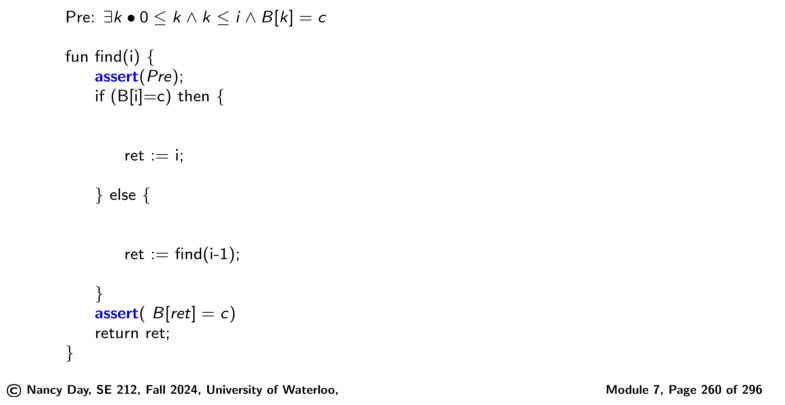
\includegraphics[width=\textwidth]{find-recursive.pdf}
I've translated the code into Dafny, and you'll find it in \texttt{dafny/FindRecursive.dfy}.
Your job is to add the correct \texttt{requires} and \texttt{ensures} clauses for this method.
With these clauses, the method must pass Dafny verification.
You don't need to make any changes to the implementation for this question.

\lstinputlisting[language=dafny]{skel/dafny/FindRecursive.dfy}


\section*{Question 4: Small Dafny Problems (15 points)}
For this question, you will have to verify three methods
in Dafny.

All files for this question are in the \texttt{dafny} folder of
the repository.

\begin{enumerate}[label=(\alph*)]
\item \textbf{\texttt{Sqrt.dfy}}: (5 points) The file contains two methods
  \[\texttt{SqrtRoot1(N: nat) returns (r:nat)}\] and \[\texttt{SqrtRoot2(N: nat) returns (r:nat)}\]
  which compute the largest $r$ such that $r \in \mathbb{Z} \wedge r \le \sqrt{N}$.

  Provide the missing invaraints so that the methods verify (2.5 points for each method).
\item \textbf{\texttt{CalcTerm.dfy}}: (5 points) The file contains a method
  \[\texttt{CalcTerm(m:int, n:nat) returns (res:int)}\]
  The method computes $5\times m - 3\times n$ using a loop and
  operations to add 5, and subtract 1 and 3.

  Provide the missing invariants so that the
  method verifies.
\item \textbf{\texttt{SlowMax.dfy}}: (5 points) The file contains a
  method \[\texttt{SlowMax(a:nat, b:nat) returns (z:nat)}\] that computes $z =
  \max(a, b)$ via a series of increments and decrements.

  Provide the missing invariants so that the
  method verifies.

\end{enumerate}



\section*{Question 5: String Reversal (10 points)}
For this question, you will have to provide one predicate and verify one methods
in Dafny. 

All files for this question are in the \texttt{dafny} folder of
the repository.

\begin{enumerate}[label=(\alph*)]
\item \textbf{\texttt{StringRevArray}}: (10 points) The file contains a skeleton of a predicate
  \texttt{isReversed} and a method \texttt{StringReverse}.

  Provide the definition of \texttt{isReversed} and the missing invariants so that the
  method verifies.
\end{enumerate}


\section*{Question 6: Sorting (30 points)} % done; reused from last year
For this question, you will have to verify two implementations of
sorting methods in Dafny. 

All files for this question are also in the \texttt{dafny} folder of
your repository.

\begin{enumerate}[label=(\alph*)]
\item (15 points) Pancake
  sorting\footnote{\url{https://en.wikipedia.org/wiki/Pancake_sorting}}
  is a sorting technique that uses only a flip operation, in which
  elements of an array are reversed (flipped) at some position. The
  subdirectory \texttt{pancakesort} contains an implementation of the pancake
  sorting algorithm in Dafny.
  \begin{itemize}
  \item Specify and verify method \texttt{findMax} in \texttt{findmax.dfy}
  \item Specify and verify method \texttt{flip} in \texttt{flip.dfy}
  \item Specify and verify method \texttt{pancakeSort} in \texttt{PancakeSort.dfy}
  \end{itemize}
  \item
    (15 points) Quicksort\footnote{\url{https://en.wikipedia.org/wiki/Quicksort}}
    is an efficient sorting technique developed by the late Tony Hoare. The
    subdirectory \texttt{quicksort} contains an implementation of quick
    sort in Dafny.
    \begin{itemize}
      \item Write a loop invariant to complete the verification of
        \texttt{partition} method in \texttt{part.dfy}
      \item \emph{(Bonus question, max 15 points)} Complete and verify the implementation of
        \texttt{qsort} method in \texttt{QuickSort.dfy}. You might
        find Chapter~6 of \emph{The Calculus of Computation}\footnote{\url{https://link.springer.com/book/10.1007/978-3-540-74113-8}} useful for this
        problem.
    \end{itemize}
\end{enumerate}


\end{document}
